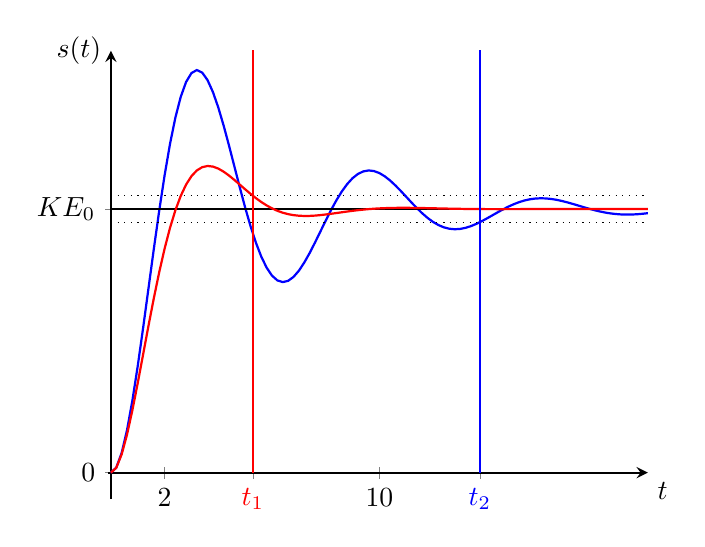
\begin{tikzpicture}                                                                                          
\pgfmathsetmacro{\a}{0.2}             % amortissement xi                                                 
\pgfmathsetmacro{\b}{0.96}            % 1-xi^2                                                           
\pgfmathsetmacro{\w}{0.979795897113}  % w_d=w_0 sqrt(1-xi^2)                                             
\pgfmathsetmacro{\p}{1.369438406}     % phi =arctan(xi/1-xi^2)                                           
\begin{axis}[                                                                                            
            axis line style = thick,                                                                             
            %height=8cm,                                                                                         
            %width=12cm,                                                                                         
            axis x line=center,                                                                                  
            axis y line=center,                                                                                  
            xmin=-0.1,                                                                                           
            xmax=20,                                                                                             
            ymin=-0.1,                                                                                           
            ymax=1.6,                                                                                            
            xlabel={$t$},                                                                                        
            ylabel={$s(t)$},                                                                                     
            xlabel style={below right},                                                                          
            ylabel style={left},                                                                                 
            xticklabels={2,\textcolor{red}{$t_1$},10,\textcolor{blue}{$t_2$}},                                   
            xtick={2,5.29,10,13.74},                                                                             
            yticklabels={0,$KE_0$,2},                                                                            
            ytick={0.001,1,2}
]
    \addplot[thick,color=blue,domain=0:20, samples=101,unbounded coords=jump]{1-((1./\w)*exp(-\a*x)*sin(deg(x)*\w+deg(\p)))};
    \addplot[thick,domain=0:20, samples=101,unbounded coords=jump]{1};
    \addplot[dotted,domain=0:20, samples=101,unbounded coords=jump]{1.05};
    \addplot[dotted,domain=0:20, samples=101,unbounded coords=jump]{0.95};
    \def\a{0.5}
    \def\b{0.75}
    \def\w{0.866025403784}                                                                                   
    \def\p{1.0471975512}
    \addplot [thick,domain=0:20, color=red,samples=101,unbounded coords=jump]{1-((1./\w)*exp(-\a*x)*sin(deg(x)*\w+deg(\p)))};
    \draw[blue,thick] (axis cs:13.74,0) -- (axis cs:13.74,2);
    \draw[red,thick] (axis cs:5.29,0) -- (axis cs:5.29,2);
    \end{axis}                                                                                               
\end{tikzpicture}                                                                                            
